\chapter{Introduction}\label{chap:Intro}
C'est dans le cadre du module \textsc{SC Project} que nous avons été amenés à effectuer le projet \textit{"Mise en place de générateurs pour des applications web"}. 
%\newline
%Nous avons porté notre choix sur ce sujet pour:....
%\newline
%1- découvrir obeo 
%\newline
%2- découvrir, dans un contexte industriel, l'ingénierie des modèles (approche vue de manière théorique dans certains cours...)
%\newline
%3- démarche MDA
%\newline
%(etc...)
%\newline
%Ce projet s'articule autour de la problématique suivante:
%\begin {center}
%\textit{"blabalblablablablabla ? (important le point d'intérrogation)"}
%\end{center}
%Pour vous décrire le déroulement du projet et répondre à cette problématique, notre rapport est scindé en "..." grandes parties. (-> annoncer brièvement le plan du rapport).


\section{L'entreprise Obeo}
\kwobeo{} est une société de service et un éditeur de logiciels \cite{obeo}.  Elle est fondée en 2005 dans la région nantaise par l'initiative de S.\textsc{Lacrampe} (directeur général), E.\textsc{Juliot} (directeur commercial) et J.\textsc{Musset} (ancien directeur technique). Elle est à l'initiative du projet Acceleo (\cf{} \cite{acceleo}), un générateur de code basé sur le framework EMF. Son expertise dans le domaine de l'ingénierie des modèles (démarche MDA) lui permet de proposer des solutions allant de la création à la refonte d'applications informatiques. 

\begin{figure}[htb]
  \centering
  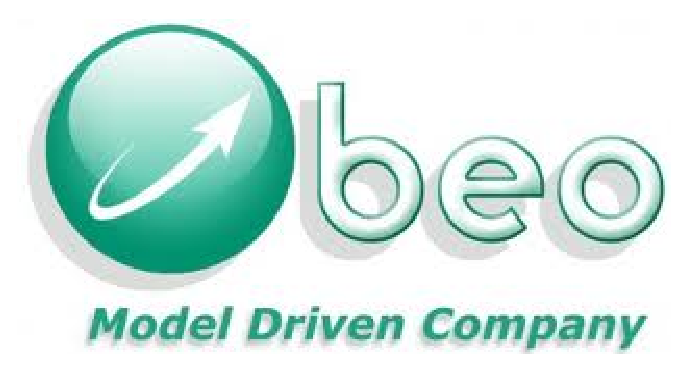
\includegraphics[scale=.4]{img/logoobeo.eps}
  \label{fig:obeo}
\end{figure}

Ces solutions proposées permettent notamment de diminuer les délais de projets et de diminuer les risques d'erreurs. Les amélioration des performances d'adaptation et d'agilité font aussi parties des objectifs des outils et méthode de la société \kwobeo{}.

La société \kwobeo{} est aussi un membre actif dans le domaine Open Source et est membre de la fondation Eclipse.


%%Infos supp : (perso je trouve qu'on en a mis assez (ALAIN) ) 

%% Après avoir été incubé par Atlanpole, consolidée dans une pépinière d'entreprise, la PME
%% déménage et s'installe dans ses locaux actuels de La Fleuriaye à Carquefou. En parallèle, pour faciliter de nouveaux
%% marchés, une agence a été ouverte en décembre 2007 à Gif-sur-Yvette (vers Paris).
%% La société Obeo développe des outils innovants pour la mise au point d'usines logiciels. Les offres Obeo
%% permettent d'industrialiser le développement d'applications informatiques (modélisation et génération de code) et leur
%% évolution (cartographie, migration, refonte). Ces offres polyvalentes sont d’ailleurs uniques sur le marché.
%% Ses clients sont principalement des Grands Comptes en informatique de gestion, en informatique embarquée et
%% également de grands intégrateurs (Thales, CEA, Atos Origin, Orange Business Services). Leur problématique est de
%% développer, maîtriser et pérenniser des patrimoines logiciels tout en réduisant les coûts, les délais et les risques. Ses
%% principaux partenaires sont la Fondation Eclipse, Alliance Libre, Atlanpole, Total développement et EADS
%% Développement. Les utilisateurs finaux de ses produits sont principalement des architectes logiciel, des chefs de
%% projets et des développeurs.



\section{Acceleo et démarche M2T}
Acceleo est un projet Open Source de la fondation Eclipse dont \kwobeo{} est à l'origine. À partir de modèles basé sur le framework EMF (\cf{} \cite{emf}), Acceleo permet de générer du code en mettant en œuvre l'approche Model Driven Architecture (MDA). Le générateur Acceleo est une implémentation de la norme de l'Object Management Group \cite{omg} pour les transformations de modèle vers texte (Model to Text : M2T).
\\\\
Le principe du Model To Text repose sur au moins trois notions essentielles :
\begin{itemize}
\item Le Méta-Modèle (ou M2) : Le M2 sert à définir les différents concepts pouvant entrer en jeu, ainsi que les relations que ces concepts entretienent entre-eux. Le M2 sert donc de base à la modélisation d'un système.
\item Le Modèle (ou M1) : Il repose sur le M2 pour décrire un système (ou une facette d'un système) en organisant les différents éléments entre eux de manière concrête, et en leur assignant un certain nombre de propriétés. Ainsi, le Modèle est utilisé pour fournir une description non-technique du réel et/ou de l'application attendue.
\item Le générateur de code : Il est utilisé pour \guim{traduire} un Modèle en code exécutable. Utilisant - la plupart du temps - un système basé sur les templates, il est configuré pour générer certaines portions de code en fonction des éléments rencontrés en parcourant le Modèle. Le générateur de code est donc utilisé pour passer d'un Modèle non-technique à une application exécutable sur la plateforme et/ou l'environnement cible. L'objectif étant qu'un même générateur de code soit capable de produire des applications différentes à partir de Modèles différents (reposant sur le même M2).\\
\end{itemize}

Le Modèle permet donc de représenter une application et son contexte en faisant abstraction de la technologie ou de la plateforme cible, à l'inverse du Générateur qui doit savoir produire une solution technique en faisant abstraction du contexte concrêt, qui est fourni par le Modèle.

% TODO Un schema pourrait etre intressant.



%%  LocalWords:  Obeo MDA Acceleo
